\documentclass{beamer}
\usetheme[titlepagelogo=img/bicocca,% Logo for the first page
		  language=italian,
		  assistantsupervisor=true,
		  secondlogo=true,
		  bullet=triangle,
		  color=red,
		  pageofpages=di,
         ]{TorinoTh}
         
\usepackage[beamer,customcolors]{hf-tikz}
\hfsetfillcolor{alerted text.fg!10}
\hfsetbordercolor{alerted text.fg}

\titlepagesecondlogo{img/ira.jpg}
\author{Federica Di Lauro}
\rel{Prof. Domenico G. Sorrenti}
\assistantsupervisor{Dott. Simone Fontana}
\title{Sistema di controllo per base robotica outdoor}
\ateneo{Università degli studi di Milano-Bicocca}
\date{24 luglio 2020}

\begin{document}

\titlepageframe % Slide iniziale

\begin{tframe}{Obiettivi}

\begin{columns}
    \begin{column}{0.45\textwidth}
        \begin{itemize}
            \item Ricerca e installazione hardware mancante
            \item Progettazione e sviluppo sistema di controllo su microcontrollore
            \item Integrazione con il framework ROS
        \end{itemize}
    \end{column}

    \begin{column}{0.45\textwidth}
        \begin{center}
            \begin{figure}
                \centering
                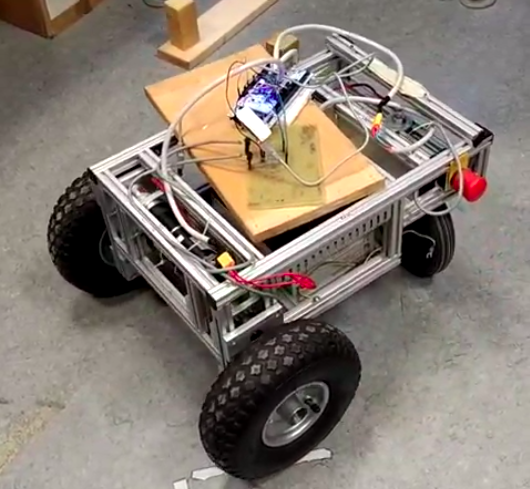
\includegraphics[width=0.9\columnwidth]{img/otto2.png}
                \caption{Base robotica Otto}
            \end{figure}
        \end{center}
    \end{column}
\end{columns}
\end{tframe}

\begin{tframe}{Infrastruttura hardware}
\begin{center}
    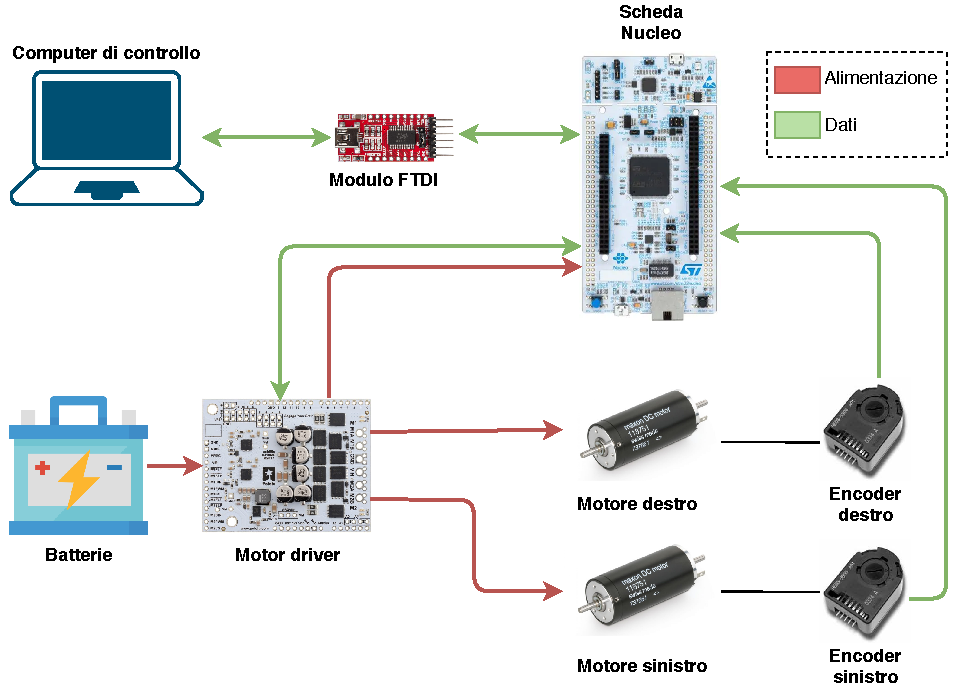
\includegraphics[width=0.8\textwidth]{img/infrastruttura.pdf}
\end{center}
\end{tframe}

\begin{tframe}{Progettazione sistema}
\begin{itemize}
\item Lato microcontrollore:
\begin{itemize}
    \item Lettura ed elaborazione dati degli encoder
    \item Controllo dei motori tramite un sistema in retroazione
    \item Comunicazione bidirezionale con un computer di controllo
\end{itemize}
\item Lato computer:
 \begin{itemize}
    \item Comunicazione con il microcontrollore
    \item Calcolo odometria
    \item Integrazione con ROS
\end{itemize}
\end{itemize}

\end{tframe}

\begin{tframe}{Progettazione software microcontrollore}
Sviluppo bare metal, senza un sistema operativo.
\begin{itemize}
    \item Task:
        \begin{itemize}
            \item Lettura encoder e invio dati
            \item Controllo PID dei motori
            \item Ricezione comandi dal computer
        \end{itemize}
    \item Periferiche utilizzate:
        \begin{itemize}
            \item Timer per interrupt periodico a 10 Hz
            \item Timer per interrupt periodico a 100 Hz
            \item UART con DMA
            \item 2 timer per lettura encoder e 1 timer per generazione PWM
        \end{itemize}
\end{itemize}

\end{tframe}

\begin{tframe}{Lettura encoder}
\begin{itemize}
    \item 2 timer in modalità \textit{encoder} per la lettura
    \item Calcolo di velocità lineare e angolare
\end{itemize}
\begin{figure}
    \centering
    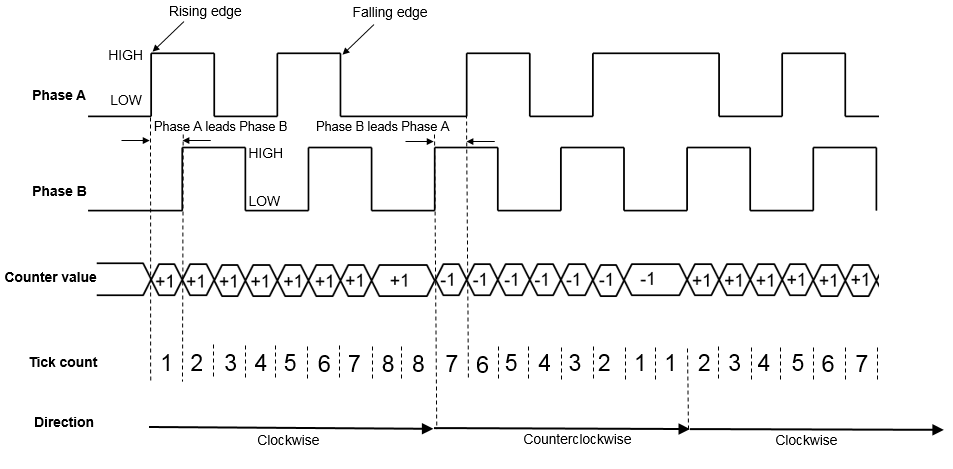
\includegraphics[width=0.9\columnwidth]{img/x4_encoder.png}
\end{figure}

\end{tframe}

\begin{tframe}{Ponte H}
Modalità di operazione \textit{sign-magnitude}:
\begin{itemize}
    \item Segnale PWM per controllo velocità
    \item Direzione controllata da un pin
\end{itemize}
    \begin{figure}
         \centering
         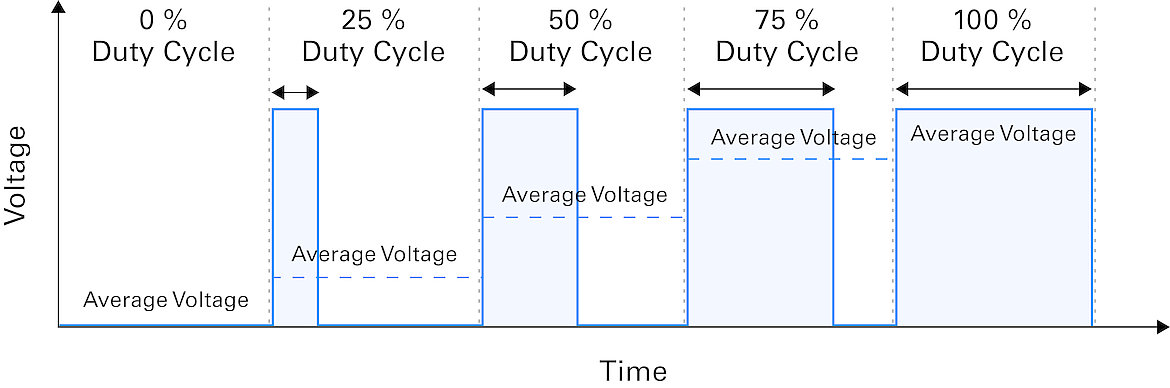
\includegraphics[width=\columnwidth]{img/pwm.jpg}
    \end{figure}
\end{tframe}

\begin{tframe}{Controllo PID}
\begin{columns}
    \begin{column}{0.5\textwidth}
        \begin{figure}
                \centering
                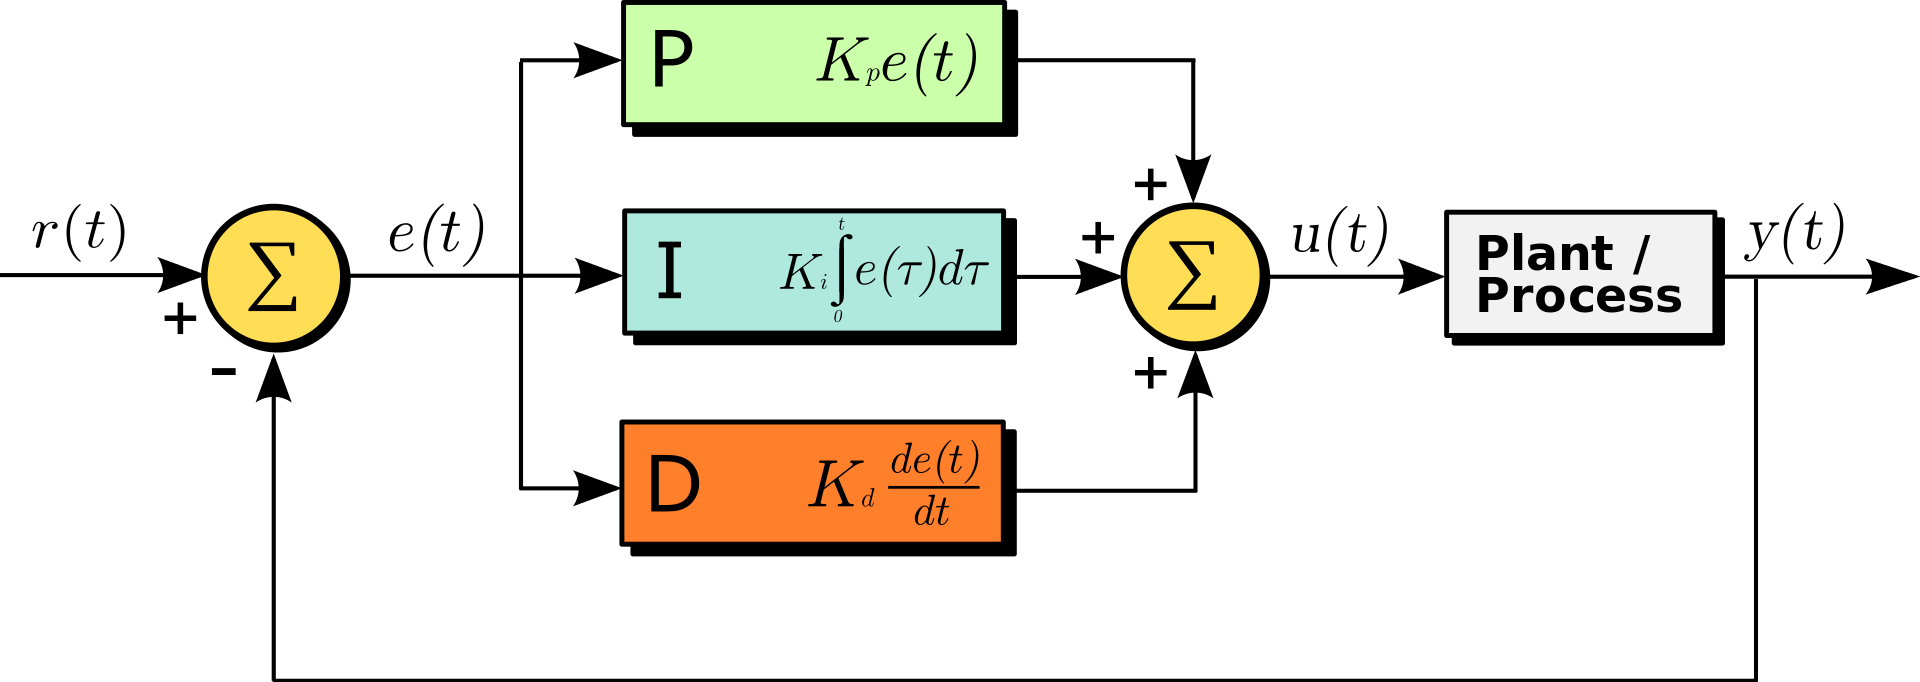
\includegraphics[width=\columnwidth]{img/pid.png}
                \caption{Schema di un generico controllore PID}
            \end{figure}
    \end{column}

    \begin{column}{0.5\textwidth}
        \begin{center}
            \begin{figure}
                \centering
                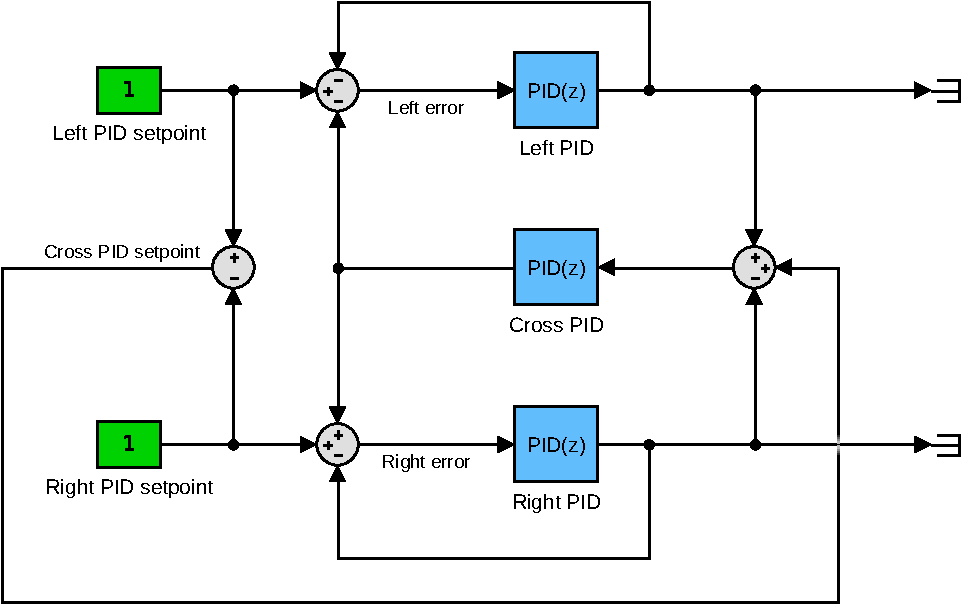
\includegraphics[width=\columnwidth]{img/crosspid.pdf}
                \caption{Schema del sistema di controllo finale}
            \end{figure}
        \end{center}
    \end{column}
\end{columns}
\end{tframe}


\begin{tframe}{Comunicazione}
Lato microcontrollore:
\begin{itemize}
    \item Periferica UART con DMA
    \item Hardware Flow Control
    \item Libreria \textit{nanopb}
\end{itemize}
Lato computer:
\begin{itemize}
    \item Modulo FTDI
    \item Libreria \textit{pyserial}
    \item Libreria \textit{Protocol Buffers}
\end{itemize}
\end{tframe}

\begin{tframe}{Nodo ROS \textit{serial\_bridge.py}}
\begin{itemize}
    \item Calcolo odometria e pubblicazione sui topic \textit{/odom} e \textit{/tf}
    \item Sottoscrizione al topic \textit{/cmd\_vel} e trasmissione a microcontrollore
\end{itemize}
\begin{figure}
         \centering
         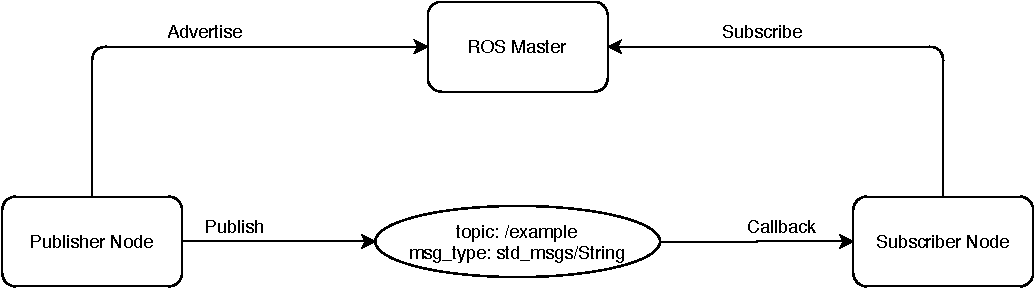
\includegraphics[width=\columnwidth]{img/ros_system.pdf}
    \end{figure}
\end{tframe}

\begin{tframe}{Testing e conclusioni}

\begin{itemize}
    \item Nodo ROS per pubblicare su \textit{/cmd\_vel} attraverso un joypad
    \item Visualizzazione odometria con RVIZ
\end{itemize}

\vspace{3mm}

\begin{figure}[h]
    \centering
    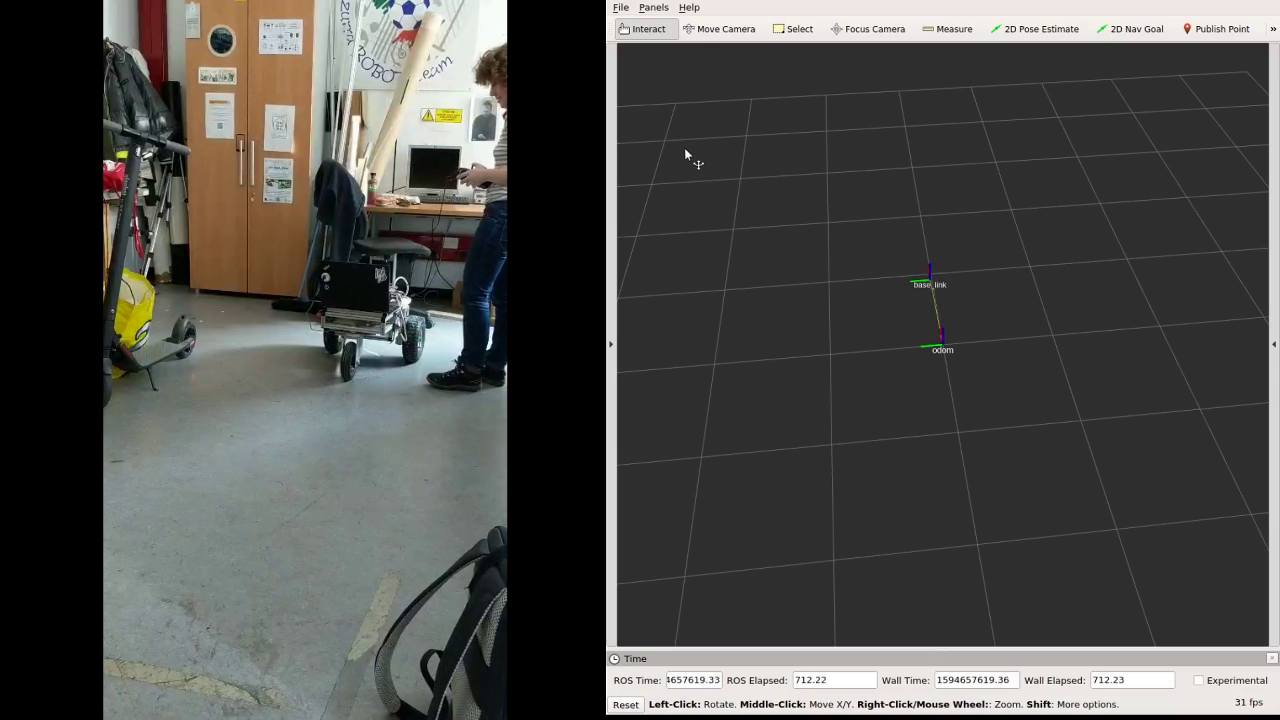
\includegraphics[scale=0.16]{img/demo.png}
\end{figure}
\centering
{\href{https://youtu.be/fEhBCXqMYPw}{Link video demo Otto}}
\end{tframe}


\begin{tframe}
    \centering
    \Huge \textsc{Grazie per l'attenzione}
    
    \vspace{5mm}
    
    \begin{columns}
        \begin{column}{0.45\textwidth}
            \begin{figure}
                \centering
                
\includegraphics[width=0.4\columnwidth]{img/bicocca.jpg}
            \end{figure}
            \begin{figure}
                \centering
                
\includegraphics[width=0.4\columnwidth]{img/ira.jpg}
            \end{figure}
        \end{column}
    
        \begin{column}{0.45\textwidth}
            \begin{center}
                \begin{figure}
                    \centering
                    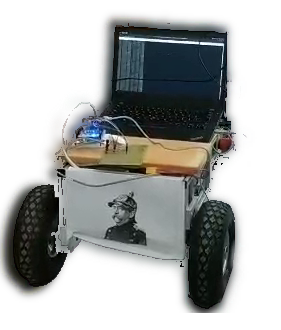
\includegraphics[scale=0.5]{img/ottofinal.png}
                \end{figure}
            \end{center}
        \end{column}
    \end{columns}
\end{tframe}

\end{document}